%-*- coding: UTF-8 -*-
\documentclass[hpyerref,UTF8,a4paper,titlepage,12pt,oneside]{ctexbook}
\usepackage{hyperref}
\usepackage{geometry}
\usepackage{xeCJK, fontspec, xunicode, xltxtra,ulem}
\usepackage{amsthm}
\usepackage{amsmath}
\usepackage{amssymb}
\usepackage{mathrsfs}
\usepackage{mathtools}
\usepackage{commath}
\usepackage{listings}
\usepackage{float}
\usepackage{xcolor}
\usepackage{mdframed}

\graphicspath{{../images/}}
\geometry{a4paper,bottom=2cm}

\title{信号采样}
\author{陈国庆}
\date{\today}

\bibliography{plain}

% 定理结构
\theoremstyle{definition}
\newtheorem{definition}{定义}[section]
\newtheorem{theorem}{定理}[section]
\newtheorem{corollary}{推论}[theorem]
\newtheorem{lemma}[theorem]{Lemma}
\renewcommand\qedsymbol{$\blacksquare$}

\begin{document}

\maketitle
\tableofcontents
\section{傅里叶级数、傅里叶变换}

\subsection{傅里叶级数}

周期为$2\pi$的连续函数$f(x)$,可展开为傅里叶级数(\textit{几乎处处}),

$$
	f(x) = \frac{a_0}{2} +\sum_{n=1}^{\infty}
	\left(
		a_n \cos nx + b_n\sin nx
	\right)
$$

其中,
\begin{align*}
	a_0 &= \frac{1}{\pi}\int_{-\pi}^{\pi} f(x)dx\\
	a_n &= \frac{1}{\pi}\int_{-\pi}^{\pi} f(x)\cos nx dx\\
	b_n &= \frac{1}{\pi}\int_{-\pi}^{\pi} f(x)\sin nx dx\\
\end{align*}

这是傅里叶级数的基本形式,可通过复指数进一步简化,考虑欧拉公式,
$$
	e^{i\theta} = \cos \theta + i \sin \theta
$$

可得,

\begin{align*}
	\cos\theta = \frac{e^{i\theta} + e^{-i\theta}}{2}\\
	\sin\theta = \frac{e^{i\theta} - e^{-i\theta}}{2i}\\
\end{align*}

所以,
\begin{align*}
	a_n \cos nx + b_n\sin nx 
		&= a_n\cdot\frac{e^{inx} + e^{-inx}}{2} + b_n\cdot\frac{e^{inx} - e^{-inx}}{2i}\\
		&= \frac{a_n - ib_n}{2}\cdot e^{inx} + \frac{a_n + ib_n}{2}\cdot e^{-inx}
\end{align*}

傅里叶级数可表示为,

\begin{align*}
	f(x) &= \frac{a_0}{2} + \sum_{n=1}^{\infty}
		\left(
			\frac{a_n - ib_n}{2}\cdot e^{inx} + \frac{a_n + ib_n}{2}\cdot e^{-inx}
		\right)\\
		&= \frac{a_0}{2} + \sum_{n=1}^{\infty}\frac{a_n - ib_n}{2}\cdot e^{inx} 
		+ \sum_{n=1}^{\infty}\frac{a_n + ib_n}{2}\cdot e^{-inx}\\
		&= \frac{a_0}{2} + \sum_{n=-\infty}^{-1}\frac{a_{-n} - ib_{-n}}{2}\cdot e^{-inx} 
		+ \sum_{n=1}^{\infty}\frac{a_n + ib_n}{2}\cdot e^{-inx}\\
		&= \sum_{n=-\infty}^{\infty}c_ne^{-inx}
\end{align*}

将$n$从正整数扩展到整数集合,得到了简洁的复指数表示。但还是不够简洁,因为系数$c_n$需分段表示,

\begin{align*}
	c_n &= \frac{a_n + ib_n}{2}, \quad n=1,2,3,\dots\\
	c_n &= \frac{a_0}{2}, \quad n=0\\
	c_n &= \frac{a_n - ib_n}{2}, \quad n=-1,-2,-3,\dots
\end{align*}

考虑$n$为正整数的场景,
\begin{align*}
	c_n &= \frac{a_n + ib_n}{2}\\
		&= \frac{1}{2\pi}
			\left[
				\int_{-\pi}^{\pi}f(x)\cos nx dx + i\int_{-\pi}^{\pi}f(x)\sin nx dx
			\right] \\
		&= \frac{1}{2\pi}\left[
			\int_{-\pi}^{\pi}f(x)
			\left(
				\frac{e^{inx}+e^{-inx}}{2}
			\right) dx 
			+ i\int_{-\pi}^{\pi}f(x)
			\left(
				\frac{e^{inx} -e^{-inx}}{2i}
			\right) dx
		\right]\\
		&=\frac{1}{2\pi}\int_{-\pi}^{\pi}f(x)e^{inx}dx
\end{align*}

当$n$为负整数时,显然$c_{-n} = c_n$,级数进一步简化为,

\begin{align}
	f(x) &= \sum_{n=-\infty}^{\infty}c_n e^{-inx}\\
	c_n &= \frac{1}{2\pi}\int_{-\pi}^{\pi}f(x)e^{inx}dx
\end{align}


若$f$的周期为$2L$,对应积分区间$[-L,L]$,令$z = \frac{\pi}{L}x$的周期为$2\pi$,对应傅里叶级数为,

$$
	f(x) = f(\frac{L}{\pi}z) = g(z)
$$

可验证,$g(z)$的周期为$2\pi$,作傅里叶展开可得,
\begin{equation}\label{f_series_form1}
	\begin{aligned}
		f(x)= &\sum_{n=-\infty}^{\infty}c_ne^{-in\frac{\pi}{L}x}\\
		c_n =& \frac{1}{2L}\int_{-L}^L f(x) e^{in\frac{\pi}{L}x}dx
	\end{aligned}
\end{equation}
因为$c_n = c_{-n}$,也可表示为,

\begin{equation}
	\begin{aligned}\label{f_series_form2}
		f(x)= &\sum_{n=-\infty}^{\infty}c_ne^{in\frac{\pi}{L}x}\\
		c_n =& \frac{1}{2L}\int_{-L}^L f(x) e^{-in\frac{\pi}{L}x}dx
	\end{aligned}
\end{equation}

傅里叶变换常解释为把一个连续信号分解为不同频率的正余弦信号叠加,分量$c_ne^{-in\pi x/L}$,表示频率为$2L/n$的信号的幅度为$c_n$。

\subsection{傅里叶变换}

	傅里叶级数能把周期信号分解为各种频率的正余弦信号,但非周期信号则无法分解,但我们又想了解非周期信号的频率成分,如此便有\textit{傅里叶变换}。\\

	非周期信号,可以认为周期无限大,即$L\rightarrow \infty$,

	(\ref{f_series_form2})式可重写为,
	$$
		2L c_n = \int_{-L}^L f(x) e^{-in\frac{\pi}{L}x}dx
	$$

	$n$可取任意值,当$L\rightarrow \infty$时,$n/2L$是一个连续变量,记为$\omega$,实际就是频率分量;则上式重写为
	$$
		2L c_n = \int_{-L}^L f(x) e^{-i2\pi\omega x}dx
	$$	

	两边取极限,

	$$
		\lim_{L\rightarrow\infty} 2L c_n = \lim_{L\rightarrow\infty} \int_{-L}^L f(x) e^{-i2\pi\omega x}dx
	$$	

	只要$f$符合\textit{绝对可积},右边极限是存在的,则左边极限也存在,且是$\omega$的函数,记为$\hat{f}(\omega)$,
	
	\begin{equation}
		\hat{f}(\omega) =  \int_{-\infty}^{\infty} f(x) e^{-i2\pi\omega x}dx\label{f_trans}
	\end{equation}

	$\hat{f}$为函数$f$的\textit{傅里叶变换},$\hat{f}$的变量是频率$\omega$,值是该频率对应的幅度。\\

	\textit{\textbf{绝对可积}}条件,
	$$
		\int_{-\infty}^{\infty} |f(x)|dx < \infty
	$$

	同样,如果已知$\hat{F}$,可以通过逆变换得到原始信号$f$,

	\begin{equation}
		f(x) =  \int_{-\infty}^{\infty} f(\omega) e^{i2\pi\omega x}d\omega\label{inver_f_trans}
	\end{equation}

	常用$\mathcal{F},\mathcal{F}^{-1}$表示傅里叶变换及逆变换,则上述变换可简记为,
	\begin{align*}
		\hat{f}(\omega) &= \mathcal{F}(f) = \int_{-\infty}^{\infty} f(x) e^{-i2\pi\omega x}dx\\
		f(x) &= \mathcal{F}^{-1}(\hat{f}) = \int_{-\infty}^{\infty} f(\omega) e^{i2\pi\omega x}d\omega
	\end{align*}

	\textit{在不同的文献中,逆变换前面可能出现$\frac{1}{2\pi}$系数,这个系数是否存在于指数中是否包含$2\pi$有关,如果指数中包含,则系数中没有,反之亦然。}

\subsection{傅里叶变换性质}	
	\subsubsection*{1、线性} 
		$$
			\mathcal{F}(\alpha f + \beta g) = \alpha \mathcal{F}(f) + \beta \mathcal{F}(g)
		$$
	\subsubsection*{2、时域平移相当于频域旋转}
		$$
			\mathcal{F}(f(x+a)) = e^{-j2\pi\omega a}\mathcal{F}(f)
		$$
	\subsubsection*{3、尺度性质}
		$$
			\mathcal{F}(f(ax)) = \frac{1}{|a|}\hat{f}(\frac{\omega}{a})
		$$

		据此性质可知,当$a>0$时,
		$$
			\mathcal{F}(\mathop{sinc}(2ax)) = \frac{1}{2a}\mathcal{F}(\mathop{sinc}(\frac{x}{2a}))
		$$

		是一个定义在$[-a,a]$,值为$\frac{\pi}{2a}$的窗函数。

	\subsubsection*{4、时域卷积相当于频域乘积,时域乘积相当于频域卷积}
		\begin{align*}
			\mathcal{F}(f \otimes g) &= \mathcal{F}(f) \mathcal{F}(g)\\
			\mathcal{F}(fg) &= \mathcal{F}(f) \otimes \mathcal{F}(g)
		\end{align*}

		此性质带来极大的便利,比如时域卷积不好计算,可以计算频域乘积,然后做逆傅里叶变换:
		$$
			f*g =\mathcal{F}^{-1}\left(\mathcal{F}(f) \mathcal{F}(g)\right)
		$$
	\subsubsection*{5、Parseval等式,又称能量守恒}
		\begin{equation}\label{parseval_eq}
			\begin{aligned}
				\int |f(x)|^2dx &= \int |\hat{f}(w)|^2d\omega\\
				\int f(x)g(x)dx &= \int \mathcal{F}(f)\mathcal{F}(g)d\omega\\
				\int \left|f(x) - g(x)\right|^2dx &= \int \left|\hat{f}(x) - \hat{g}(x)\right|^2d\omega
			\end{aligned}
		\end{equation}
		
		最后一个式子表明,时域频域的$L_2$距离保持不变。
	\subsubsection*{6、$n$阶导数的傅里叶变换}
		$$
			\mathcal{F}(f^{(n)}) = (i2\pi\omega)^n \hat{f}(\omega)
		$$
	\subsubsection*{7、周期性}
		$$
			\mathcal{F}^0 = I, 
			\mathcal{F}^1 = \hat{f}, 
			\mathcal{F}^2 = f(-x), 
			\mathcal{F}^3 = \mathcal{F}^{-1},
			\mathcal{F}^4 = \mathcal{F}^0
		$$

\subsection{特殊函数及其变换}
	\subsubsection*{1、高斯函数}
		$$ f(x) = e^{-ax^2} $$

		\begin{align*}
			\hat{f}(\omega) 
				&= \int_{-\infty}^{\infty} e^{-ax^2}\cdot e^{-i2\pi\omega x}dx\\
				&= \int_{-\infty}^{\infty}  
					\exp\left\lbrace
						-a\left(
							x^2 + 2\frac{i\pi\omega}{a} x
						\right)
					\right\rbrace dx\\
				&=  \int_{-\infty}^{\infty}  
					\exp\left\lbrace
						-a\left(
							x^2 + 2\frac{i\pi\omega}{a} x + \frac{i\pi\omega}{a}
						\right)^2 + a\left(\frac{i\pi\omega}{a}\right)^2
					\right\rbrace dx\\
				&= C\int_{-\infty}^{\infty} \exp \left\lbrace
						-a\left(
							x+\frac{i\pi\omega}{a}
						\right)^2
					\right\rbrace dx\quad ,
					\left(
						C = \exp\left\lbrace
								-\frac{(\pi\omega)^2}{a}
					\right\rbrace\right)\\
				&= C\int_{-\infty}^{\infty} \exp \left\lbrace
						-\left(
							\sqrt{a}x+\frac{i\pi\omega}{\sqrt{a}}
						\right)^2
					\right\rbrace dx\\
				& = C\int_{-\infty}^{\infty} 
							e^{-u^2}
					 \frac{1}{\sqrt{a}}dx\quad , \left(u = \sqrt{a}x+\frac{i\pi\omega}{\sqrt{a}}\right)\\
				&= \frac{\sqrt{2\pi}C}{\sqrt{a}}
					\frac{1}{\sqrt{2\pi}}\int_{-\infty}^{\infty} e^{-u^2}dx\\
				&= \sqrt{\frac{2\pi}{a}}
							\exp
								\left\lbrace
									-\frac{(\pi\omega)^2}{a}
								\right\rbrace
		\end{align*}

		高斯函数傅里叶变换还是高斯函数,无论在时域还是频域,高斯函数形式都不变。
	\subsubsection*{2、窗函数}

		标准窗函数定义为,
		$$
			\chi(x) = 
			\begin{cases}
				1,& x \in [-\frac{1}{2},\frac{1}{2}]\\
				0,& \text{others}
			\end{cases}
		$$

		以及带参数的形式,
		\begin{equation}\label{rect_pram_trans}
			\chi_{[-B,B]}(x) = \chi(\frac{x}{2B})
		\end{equation}

		\begin{align*}
			\hat{\chi}(\omega) 
				& = \int_{-\infty}^{\infty} f(x) e^{-i2\pi\omega x}dx\\
				& = \int_{-\frac{1}{2}}^{\frac{1}{2}} e^{-i2\pi\omega x}dx\\
				& = -\frac{1}{i2\pi\omega}
					\int_{-\frac{1}{2}}^{\frac{1}{2}} e^{-i2\pi\omega x}d(-i2\pi\omega x)\\
				& = \frac{1}{i2\pi\omega}\int_{-i\pi\omega}^{i\pi\omega} e^{u}d(u)\\
				&= \frac{1}{i2\pi\omega}\left(e^{i\pi\omega} - e^{-i\pi\omega}\right)\\
				&=\mathop{sinc}(\omega)
		\end{align*}

		窗函数的傅里叶变换是$\mathop{sinc}$函数。由缩放性质,

		\begin{align*}
			\hat{\chi}_{[-B,B]}(\omega) &= 2B\mathop{sinc}(2B\omega)
		\end{align*}

		根据周期性,
		$$
			\chi(-x) =\mathcal{F}^2(\chi) = \mathcal{F}(\mathop{sinc}) 
		$$
		
		sinc函数的傅里叶变换为窗函数。

	\subsubsection*{3、sinc函数}

		一般$\mathop{sinc}$函数定义为,
		$$
			f(x) =\frac{\sin x}{x}
		$$

		也经常用下面的形式,

		$$
			\mathop{sinc}(x) =f(\pi x) = \frac{\sin \pi x}{\pi x}
		$$

		$x = 0$是sinc函数的奇点,

		$$
			\lim_{x\rightarrow 0} \frac{\sin x}{x} = 1
		$$

		补充$f(x) = 1$,使得函数没有奇点。\\

		\begin{figure}[H]
			\begin{center}
				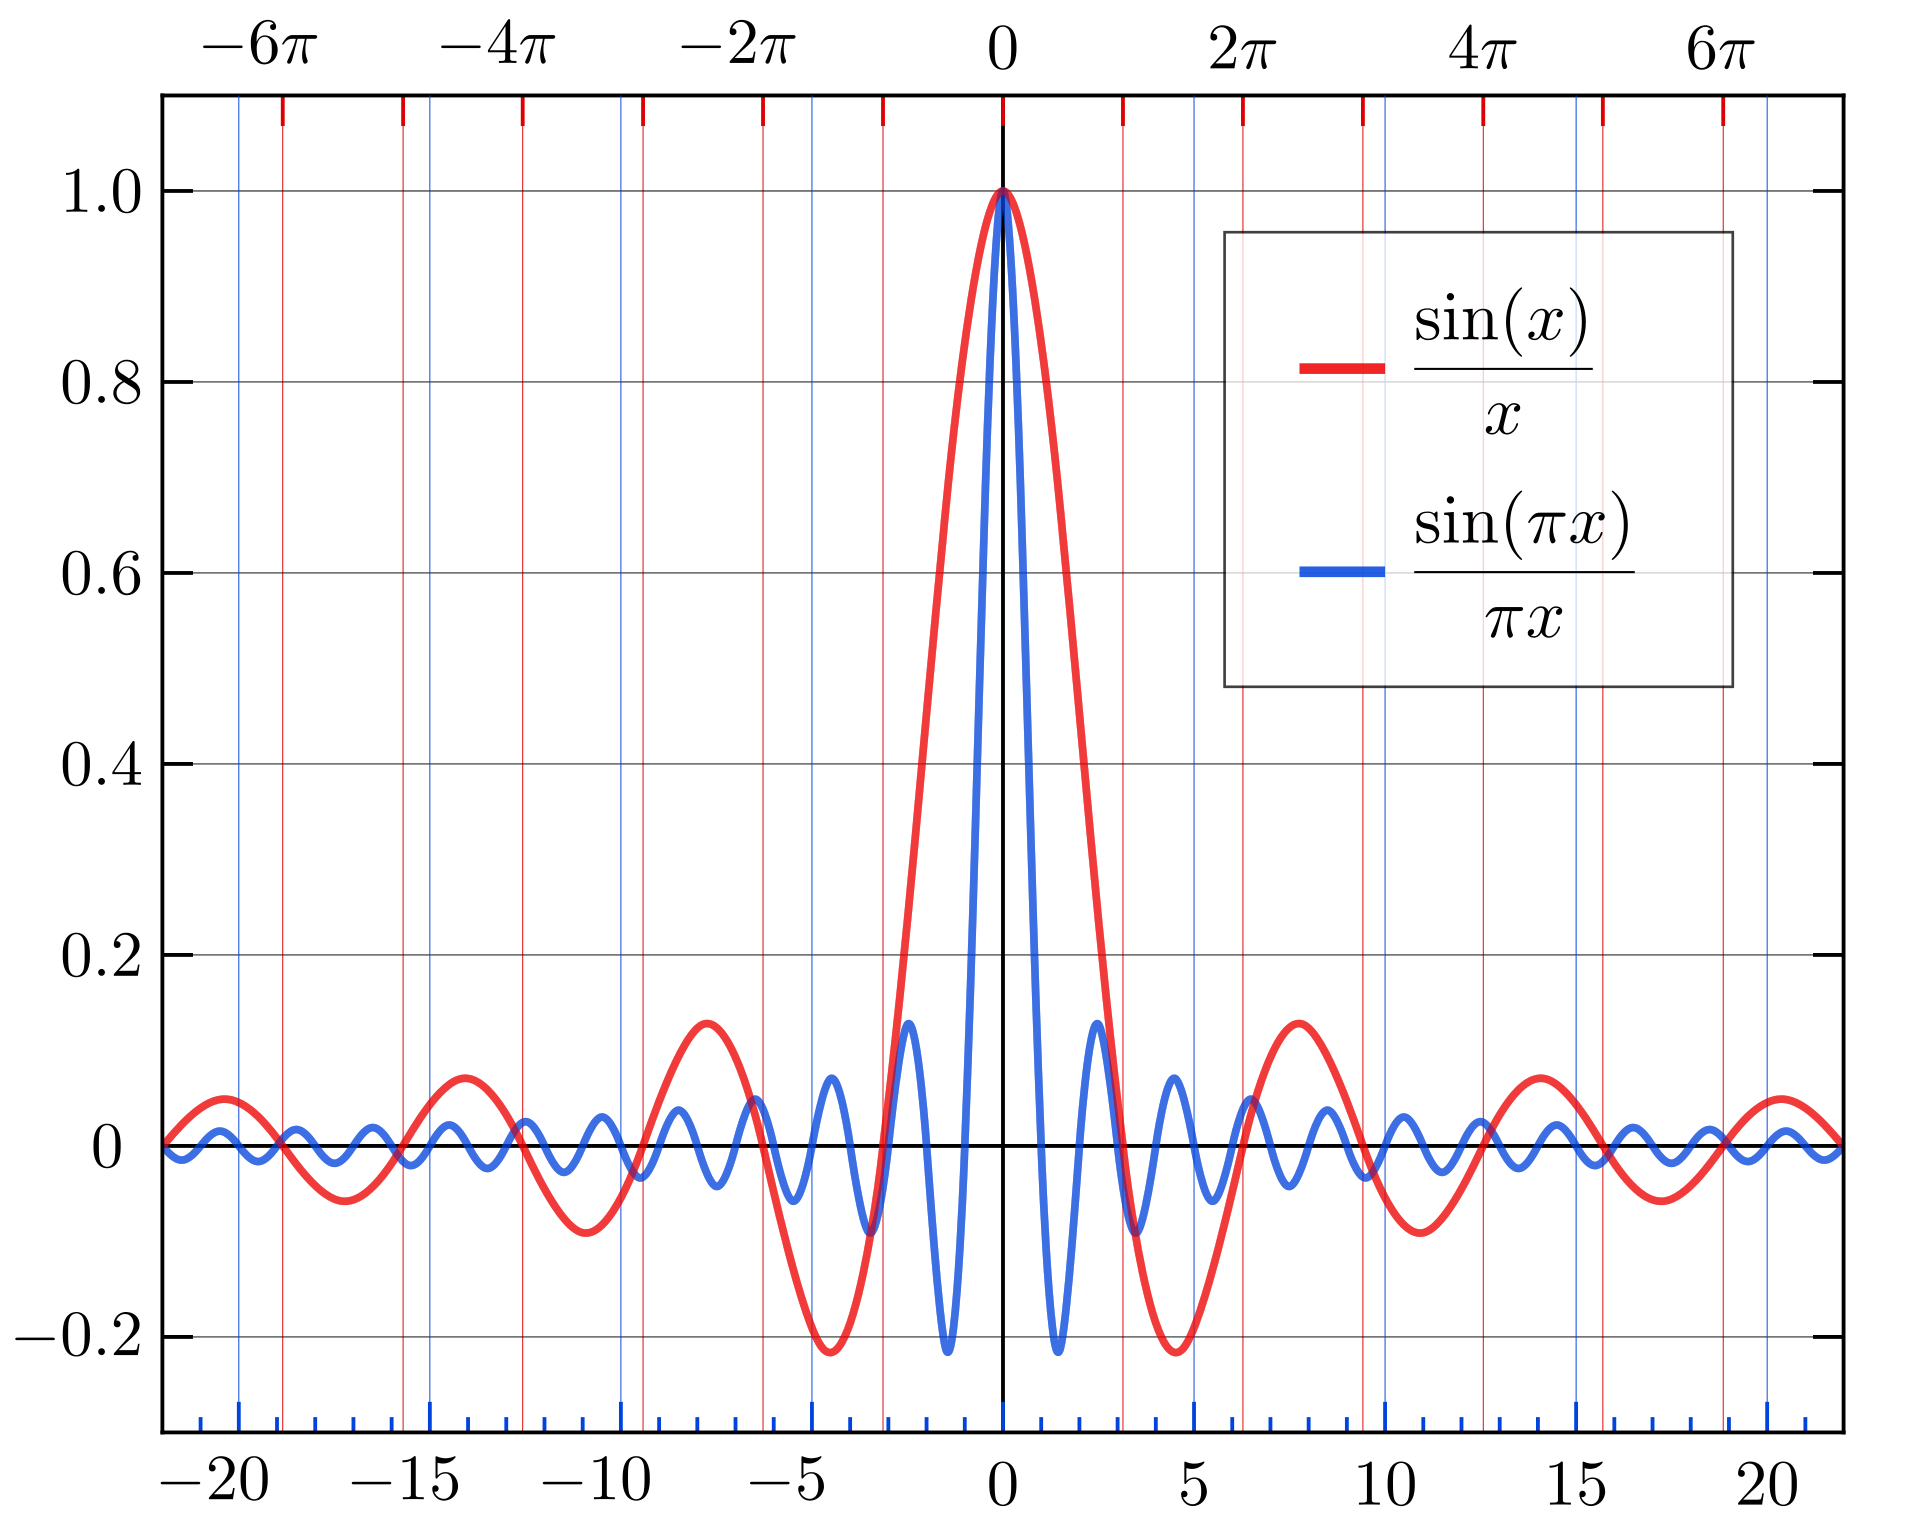
\includegraphics[width=0.8\textwidth]{./images/sinc_graph.png}
			\end{center}
		\end{figure}

		通过周期性已知sinc函数的傅里叶变换是窗函数,下面介绍下直接求解过程。\\


		考察下以下定积分(sinc是偶函数),

		$$
			J = \int_{-\infty}^{\infty} \frac{\sin x}{x}dx = 2\int_{0}^{\infty} \frac{\sin x}{x}dx
		$$

		构造$x$的积分表示,
		$$
			\frac{1}{x} = \int_0^\infty e^{-ax}da
		$$

		代入计算,

		$$
			J = 2\int_{0}^{\infty} \sin x \int_0^\infty e^{-ax}da dx = 2\int_{0}^{\infty}\int_{0}^{\infty}\sin x e^{-ax} dx da
		$$

		\begin{align*}
			K &= \int_{0}^{\infty}\sin x e^{-ax} dx\\
				&= -\int_{0}^{\infty}e^{-ax} d\cos x\\
				&= -\cos x \cdot e^{-ax}\Big|_0^{\infty} + \int_{0}^{\infty}\cos x de^{-ax}\\
				&= 1 - a \int_0^\infty \cos x e^{-ax} dx\\
				&= 1 - a^2K
		\end{align*}

		所以
		$$
			K = \frac{1}{1+ a^2}
		$$

		$$
			J = 2\int_{0}^{\infty} \frac{1}{1+a^2}da = 2\arctan(a)\Big|_0^\infty = \pi
		$$

		由此可知,
		\begin{equation}
			\int_{-\infty}^{\infty} \mathop{sinc}(x)dx = \int_{-\infty}^{\infty} \frac{\sin \pi x}{\pi x}dx = \frac{J}{\pi} = 1 \label{sinc_int_value1}
		\end{equation}

		sinc函数的傅里叶变换,
		\begin{align*}
			\mathcal{F}(\mathop{sinc}) 
				& = \int_{-\infty}^{\infty} \frac{\sin \pi x}{\pi x} e^{-i2\pi\omega x}dx\\
				&= \int_{-\infty}^{\infty} \frac{\sin \pi x}{\pi x} \cos 2\pi\omega x dx + i \int_{-\infty}^{\infty} \frac{\sin \pi x}{\pi x} \sin 2\pi\omega x dx\\
				&= 2 \int_0^\infty\frac{\sin \pi x  \cdot \cos 2\pi\omega x}{\pi x} dx\\
				&= \int_0^\infty\frac{\sin (1 + 2\omega)\pi x  + \sin (1 - 2\omega)\pi x}{\pi x} dx\\
				&= \int_0^\infty\frac{\sin (1 + 2\omega)\pi x }{\pi x} dx
				+ \int_0^\infty\frac{\sin (1 - 2\omega)\pi x}{\pi x} dx
		\end{align*}

		由(\ref{sinc_int_value1})知,
		\begin{equation}
			\mathcal{F}(\mathop{sinc})(\omega) = \chi(\omega)\label{sinc_f_trans}
		\end{equation}

		sinc函数的傅里叶变换是窗函数。

	\subsubsection*{4、Dirac $\delta$函数}
	
		Dirac $\delta$函数是一个广义函数,满足如下条件,
		\begin{enumerate}
			\item 基础性质
				\begin{equation}\label{delta_func}
				\begin{aligned}
					\delta(x) = 
					\begin{cases}
						\infty, &x=0\\
						0, &x\neq 0
					\end{cases}
				\end{aligned}				
				\end{equation}

			\item 积分性质
				$$
					\int_{-\infty}^{\infty}\delta(x)dx = 1
				$$			
		\end{enumerate}

		$\delta$函数的积分具有\textit{选择性},

		\begin{align*}
			\int_{-\infty}^{\infty}\delta(x-x_0)f(x)dx = f(x_0)\label{delta_selection}
		\end{align*}

		根据选择性,$\delta(x-x_0)$的傅里叶变换为,
		\begin{align*}
			\mathcal{F}(\delta(x-x_0))(\omega) 
				= \int_{-\infty}^{\infty} \delta(x-x_0) e^{-i2\pi\omega x}dx
				= e^{-i2\pi\omega x_0}
		\end{align*}

		$\delta(x)$的傅里叶变换为,$\mathcal{F}(\delta(x)) = 1$。\\


		$\delta(x)$的逆变换为,

		\begin{equation}
			\delta^\prime(x) = \mathcal{F}^{-1}(\mathcal{F}(\delta(x))) = \int_{-\infty}^{\infty}e^{i2\pi x \omega}d{\omega}\label{delta_int_form}
		\end{equation}

		这是$\delta$函数的积分形式,需验证$\delta^\prime$满足$\delta$的条件,才能确保逆变换的正确性。\\

		1、验证$0$点的值
		$$
			\delta(0) = \int_{-\infty}^{\infty} 1 d\omega = \infty
		$$

		2、验证非$0$点值
			\begin{align*}
				\delta^\prime(x) 
					&= \lim_{n\rightarrow \infty} = \int_{-n\pi}^{n\pi}e^{i2\pi x \omega}d{\omega}\\
					&= 2\lim_{n\rightarrow \infty}\int_{-n\pi}^{n\pi} \cos (2\pi x \omega) d{\omega}\\
					&=0
			\end{align*}
		
		3、验证积分
		\begin{align*}
			\int_{-\infty}^{\infty} \delta^{\prime}(x) dx 
				&= \int_{-\infty}^{\infty}\int_{-\infty}^{\infty}e^{i2\pi x \omega}d{\omega}dx\\
				&= 2\int_{-\infty}^{\infty}\left[\int_{0}^{\infty} \cos 2\pi x\omega d{\omega}\right]dx\\
				&= 2\int_{-\infty}^{\infty}\left[\lim_{N\rightarrow \infty}\int_{0}^{N} \cos 2\pi x\omega d{\omega}\right]dx\\
				&= 2\lim_{N\rightarrow \infty}\int_{-\infty}^{\infty}\frac{\sin 2\pi x N}{2\pi x}dx\\
				&= 1
		\end{align*}

		所以$\delta^\prime$的确是$\delta$函数。

	\subsubsection*{5、Dirac梳函数}

		Dirac梳函数是通过$\delta$函数平移$T$复合而成,

		\begin{equation}
			\mathop{C}(x,T) = \sum_{n=-\infty}^{\infty} \delta(x-nT) \label{dirac_comb}
		\end{equation}

		函数支撑集仅在$nT$处,所以是一$T$为周期的周期函数,

		\begin{figure}[H]
			\begin{center}
				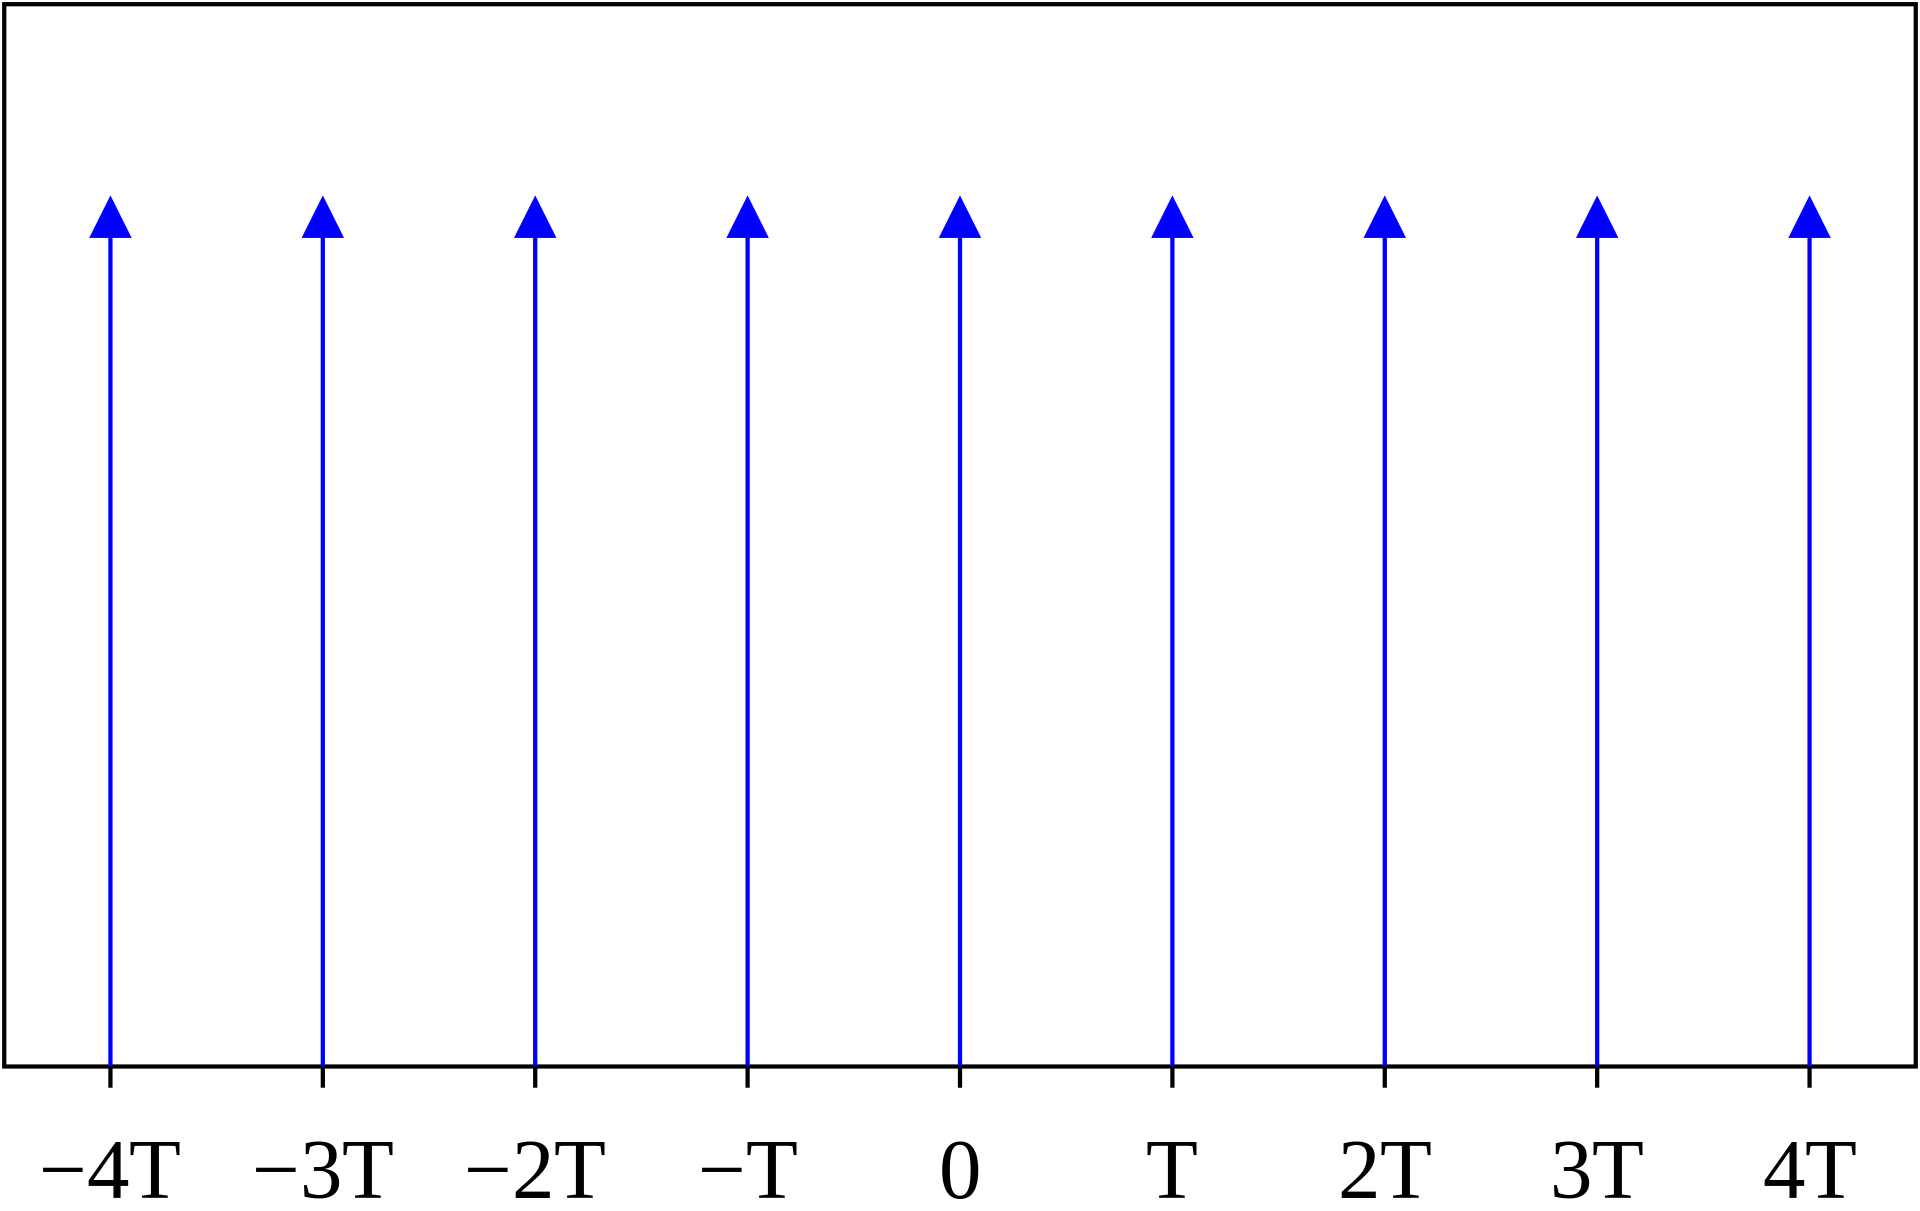
\includegraphics[width=0.8\textwidth]{./images/dirac_comb.png}
			\end{center}
			\caption{周期为$T$的$\delta$梳函数}
		\end{figure}

		梳函数可以展开为\textit{傅里叶级数},根据(\ref{f_series_form2})系数为,
		$$
			c_n = \frac{1}{T}\int_{kT-T/2}^{kT+T/2}
				\sum_{k=-\infty}^{\infty} \delta(x-kT)e^{\frac{-i2\pi n}{T}x}dx = \frac{1}{T}
		$$

		\textbf{梳函数的傅里叶级数},
		\begin{equation}
			\mathop{C}(x,T) =\frac{1}{T} \sum_{n=-\infty}^{\infty} e^{\frac{i2\pi n}{T}x} \label{delta_f_series}
		\end{equation}

		\textbf{梳函数的傅里叶变换},
		\begin{align*}
			\mathcal{F}(\mathop{C(x,T)}) 
				&= \int_{-\infty}^{\infty} \frac{1}{T} \sum_{n=-\infty}^{\infty} e^{\frac{i2\pi n}{T}x} \cdot  e^{-i2\pi\omega x}dx\\
				& = \frac{1}{T} \sum_{n=-\infty}^{\infty} \int_{-\infty}^{\infty} e^{i2\pi(\omega - \frac{n}{T}) x}dx\\
				& = \frac{1}{T} \sum_{n=-\infty}^{\infty} \delta(\omega,\frac{n}{T})\\
				& = \frac{1}{T}\mathop{C}(\omega, \frac{n}{T})
		\end{align*}

		倒数第二步,
		$$
			h(\omega) = \int_{-\infty}^{\infty} e^{i2\pi(\omega - \frac{n}{T}) x}dx
		$$

		根据分步骤积分容易计算,
		$$
			h(\omega) =
			\begin{cases}
				0, & \omega = \frac{n}{T}\\
				\infty, & \text{others}
			\end{cases}
		$$

		这实际就是$\delta(\omega,n/T)$,所以梳函数的傅里叶变换,仍然是梳函数。\\

		为什么需借助傅里叶级数计算梳函数的傅里叶变换,而非直接计算?\\

		梳函数是周期函数,不满足\textit{绝对可积}条件,无法计算傅里叶变换。分解为傅里叶级数后,每个分量都满足\textit{绝对可积}。\\

		不仅是梳函数,所有的周期函数,都应该通过这个方式计算傅里叶变换。

		\textbf{梳函数卷积},

		\begin{align*}
			g(\tau) = \mathop{C}(x,T) * f(x) = \int \mathop{C}(\tau-x,T)f(x)dx
		\end{align*}

		梳函数翻转与自身对称,所以$\mathop{C}(-x,T) = \mathop{C}(x,T)$,及
		$$
			C(\tau-x,T) = C(x+\tau,T) = \sum_{n=-\infty}^{\infty}\delta(x + \tau - nT)
		$$

		根据$\delta$函数的选择性,
		$$
			g(\tau) = \sum_{n=-\infty}^{\infty}f(\tau - nT)
		$$

		得到一个重要结论:任意函数与梳函数卷积,相当于原函数平移,对应点求和。平移,相当于对原函数做了周期沿拓。
		\begin{figure}[H]\label{comb_replica}
			\begin{center}
				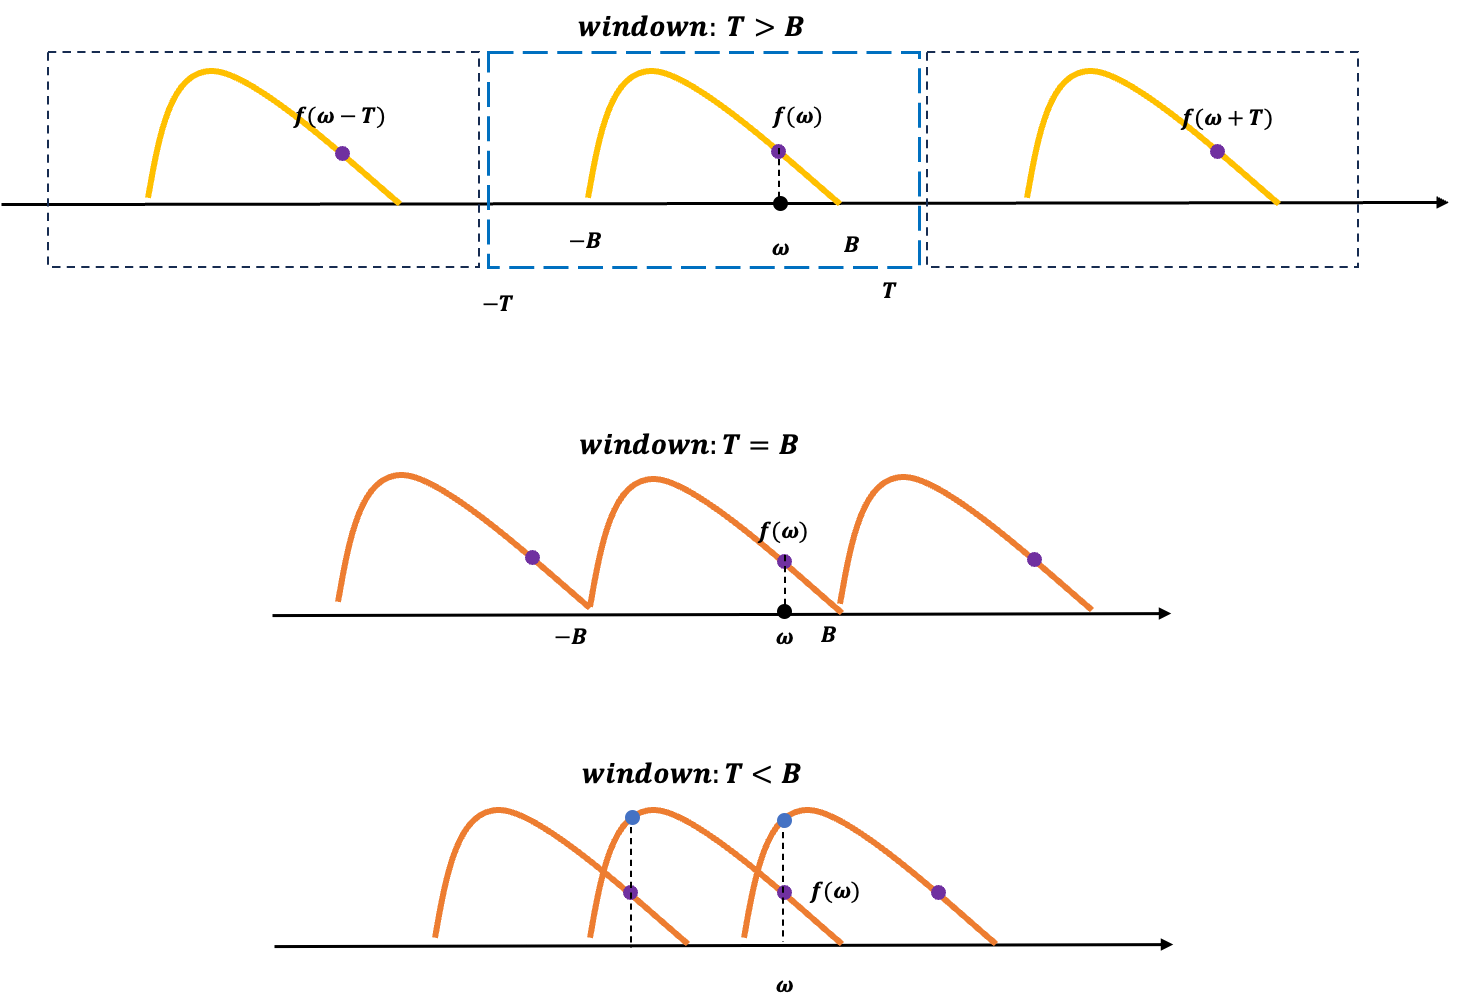
\includegraphics[width=\textwidth]{./images/comb_shift.png}
			\end{center}
			\caption{不同周期梳函数对函数的平移}
		\end{figure}

		根据上图可知,当梳函数的周期大于等于目标函数周期时,每个点对应一个函数值;否则有多个函数值,计算$g(\tau)$会出现歧义。\\

		在信号的频域中,这就是\textit{频率混叠}现象,后面会再讨论。

\subsection{逆变换证明}
	\begin{align*}
		\mathcal{F}^{-1}(\mathcal{F}(f))(x) &= \int_{-\infty}^{\infty} \hat{f}(\omega) e^{i2\pi x\omega}d\omega\\
			 &= \int_{-\infty}^{\infty} 
			 \left[
			 \int_{-\infty}^{\infty}f(t)e^{-i2\pi \omega t}dt e^{i2\pi x\omega}\right]d\omega\\
			 &= \int_{-\infty}^{\infty} f(t)
			 	\left[
			 		\int_{-\infty}^{\infty}e^{i2\pi \omega (x-t)}d\omega
			 	\right]dt
	\end{align*}

	由(\ref{delta_int_form})知,
	$
		\delta(x-t) = \int_{-\infty}^{\infty}e^{i2\pi \omega (x-t)}d\omega
	$

	$$
		\mathcal{F}^{-1}(\mathcal{F}(f))(x) = \int_{-\infty}^{\infty} f(t) \delta(x-t)dt = f(x)
	$$

	最后一步跟进$\delta$函数选择性。

\subsection{时域频域}

	时域,频域都是函数空间,通过傅里叶变换,在两个空间建立了一一映射,
	$$
		f(x) \overset{\mathcal{F}}{\rightarrow} \hat{f}(\omega) 
	$$

	我们在时域定义函数乘法运算,在频域定义卷积预算,这两个运算在$\mathcal{F}$映射下也是对应的,所以粗略来说,时域与频域如果看作群的话,两个群是\textit{同构}的。\\

	代数上,同构群认为是相同的,所以在时域上分析信号随时间变化,等价于频域上分析信号随频率的变化,而后者经常更容易一些。\\

	当然这两个空间构不成群,因为不是所有的函数都有反函数,但这并不在重要。

\section{Shannon采样定理}

\subsection{采样定理}

如果已知某个连续函数$f(x)$一些离散值$f(x_i)(i=1,2,\dots)$,能否恢复出完整的$f(x)$?\\

如果$f(x)$本身及对应的傅里叶变换符合一定的条件,这是可以做到的,有如下\textit{Shannon采样定理},

\begin{theorem}\label{th:discret_rep}
	\textbf{Shannon采样定理}\quad 若$f \in L_{1}(\mathbb{R})$,$\hat{f}$的支撑集为$[-B,B]$($B$称为\textit{Nyquist 频率}),则
	\begin{equation}\label{shannon_th}
		f(x) = \sum_{n \in \mathbb{Z}} f\left(\frac{n}{2B}\right) \mathop{sinc}\left(2B\left(x-\frac{n}{2B}\right)\right)
	\end{equation}
\end{theorem}

\begin{proof}
	$\hat{f}$定义域是$[-B,B]$,因此可周期延拓到整个实数轴上。系数$c_n$(\ref{f_series_form1}),
	\[
		c_n = \frac{1}{2B} \int_{-B}^B \hat{f}(x) e^{\frac{i2\pi  n x}{2B}}dx = \frac{1}{2B}f\left(\frac{-n}{2B}\right)
	\]
	
	对应的傅里叶技术展开为,
	\begin{equation*}
		\hat{f}(\omega) = \sum_{n \in \mathbb{Z}}\frac{1}{2B}f\left(\frac{n}{2B}\right)e^{\frac{-i2\pi  n \omega}{2B}} \quad\left(x \in [-B,B]\right)
	\end{equation*}

	通过窗函数把定义域扩展到$(-\infty,\infty)$,
	
	\begin{equation}\label{eq:freq_series}
		\hat{f}(\omega) = \sum_{n \in \mathbb{Z}}\frac{1}{2B}f\left(\frac{n}{2B}\right)
		\chi_{[-B,B]}(\omega)
		e^{\frac{-i2\pi  n \omega}{2B}}
	\end{equation}

	结合傅里叶变换的性质:
	\begin{itemize}
		\item 周期性:$f(-x) = \mathcal{F}(\hat{f})(x)$
		\item 窗函数变换到sinc函数:$\hat{\chi}_{[-B,B]}= 2B\mathop{sinc}(2Bx)$
		\item 旋转对应平移:乘以$e^{\frac{-i2\pi  n \omega}{2B}}$等价平移$-\frac{n}{2B}$
	\end{itemize}

	对(\ref{eq:freq_series})两边做傅里叶变换可得(\ref{shannon_th})。
\end{proof}

	Shannon采样定理表明,$f(x)$可以用$\mathop{sinc}$函数基分解,系数为离散采样点;对比傅里叶级数,用正余弦函数基分解,系数为积分值。\\

	一般函数基分解出的系数,都有基本身有关,而$\mathop{sinc}$函数基产生的系数竟然与基本身无关,这真是一个令人吃惊的结论。

\subsection{Nyquist采样频率}
	
	用任意的Nyquist频率$B_0$采样,按(\ref{eq:freq_series})的方式得到,
	$$
		\hat{h}(\omega) = \sum_{n \in \mathbb{Z}}\frac{1}{2B_0}f\left(\frac{n}{2B_0}\right)
		\chi_{[-B_0,B_0]}(\omega)
		e^{\frac{-i2\pi  n \omega}{2B_0}}
	$$

	\textbf{1、$B_0 < B$}, 对任意$|\omega| \in [B_0,B]$,都有$\hat{h}(\omega) =0 \ne \hat{f}(\omega)$,此时$\hat{h}$无法重建出$f(x)$\\

	\textbf{2、$B_0 > B$},扩展$\hat{f}$的支撑集到$[-B_0,B_0]$,构建函数$\tilde{h}$,
	$$
		\tilde{h}(\omega) = \chi_{[-B,B]}\hat{f}(\omega), \quad\omega \in [-B_0, B_0] 
	$$

	将$\tilde{h}$以$2B_0$作周期延拓,展开傅里叶级数的系数为,
	\begin{align*}
		c_n
			&= \frac{1}{2B_0}\int_{-B_0}^{B_0} \chi_{[-B_0,B_0]}\hat{f}(x) e^{\frac{i2\pi nx}{2B_0}}dx\\
			&= \frac{1}{2B_0}\int_{-B_0}^{B_0} \chi_{[-B,B]}\hat{f}(x) e^{\frac{i2\pi nx}{2B_0}}dx\\
			&= \frac{1}{2B_0}\int_{-B}^{B} \hat{f}(x) e^{\frac{i2\pi nx}{2B_0}}dx\\
			&= \frac{1}{2B_0}f\left(\frac{n}{2B_0}\right)
	\end{align*}

	对比可知,$\hat{h} = \tilde{h}$,$\hat{h}$是$\hat{f}$支撑集扩大到$[-B_0,B_0]$后的傅里叶级数。\\

	$\hat{h}$的逆变换,根据周期性,

	\begin{align*}
		h(-x) &= \mathcal{F}(\hat{h})(\omega) 
			= \left(\int_{-B_0}^{-B} + \int_{-B}^{B} + \int_{B}^{B_0} \right)
			\chi_{[-B,B]}\hat{f}(\omega) e^{-i2\pi \omega x}d\omega
			 = f(-x)
	\end{align*}
	
	\textit{当$B_0\ge B$,通过Shannon采样定理构造的函数,能点点收敛到原函数。也就是采样频率区间至少是$2B$。}\\

	证明过程蕴含了一个反直觉的结论:

	\begin{itemize}
		\item 时域空间,高采样频率对应更密集的样本,对信号重建\underline{\textit{应该有}}帮助
		\item 频域空间,高采样频率只是扩展了频谱支撑集,对频谱重建\underline{\textit{没有}}帮助
	\end{itemize}
	
	时域与频域是同构,在频域没有帮助的操作,对应到时域就是冗余计算。\\

	当然在具体实现时,因为信号存在噪音、丢失等情况,更密集的采样有助于平滑这些异常值。\\

	一般不知道信号的最高频率,经常根据经验估一个采样频率,估低了高频信息会丢失,无法准确重建;估高了又会造成冗余计算,这是一个权衡的过程。

\subsection{sinc正交基}
	
	Shannon采样定理(\ref{th:discret_rep})揭示了一个深刻的结论:对频域有\textit{紧支撑}的连续函数,可以sinc函数基分解,分量是原函数的离散值。\\

	实际上sinc函数基是标准正交基,下面是证明过程。\\

	注意一个通过傅里叶变换计算积分的技巧,
	$$
		\int_{-\infty}^{\infty} f(x) dx = \hat{f}(0)
	$$

	令
	$$
		J(n,\omega) = \mathcal{F}(\mathop{sinc}(x)\mathop{sinc}(x+n)) (\omega)\quad (n\in \mathbb{Z})
	$$
	只要证明$J(n,0)=0,J(0,0) = 1$即可。

	\begin{align*}	
		J(n,\omega) &= \mathcal{F}(\mathop{sinc}(x)) \otimes \mathcal{F}((\mathop{sinc}(x+n)) \\
		& = \chi(\omega) \otimes e^{-i2\pi \omega n} \chi(\omega) \\
		& = \int_{-1/2}^{1/2} e^{-i2\pi (\omega -x) n} dx\\
	\end{align*}

	$$
		\begin{aligned}
				J(n,0)&= \int_{-1/2}^{1/2} e^{i2\pi nx } dx =0 \\
				J(0,0)&= \int_{-1/2}^{1/2} dx = 1		
		\end{aligned}
	$$

	在\textit{有限维线性空间}中,经常选择不同的基向量作为坐标系,两个坐标系之间存在一个\textit{线性变换},通常用一个矩阵表示。\\

	在\textit{无限维函数空间}中,也经常选择不同的函数基作为坐标系,比如傅里叶基、sinc基、多项式基及小波基等,这些坐标系之间存在某种\textit{非线性变换},并没有统一的表示方式,这是函数空间比线性空间复杂的地方。\\

	通过不同的基函数,能观察到函数不同的性质,
	\begin{itemize}
		\item 傅里叶基,能观察到信号频率的构成情况;
		\item sinc函数基,能观察到函数通过离散点重建的过程;
		\item 小波基,能观察到随观察尺度变化的函数响应
	\end{itemize}

	机器学习中的核心工作可总结为数据降维,实际就是以数据驱动的方式学习出合适的坐标系。这种坐标系只是以神经网络的形式而存在,无法解析刻画,与前面提到的各种基函数坐标系是完全不同的。
	




	






\section{信号采样}

信号采样主要目的是把连续信号给存入计算机进行分析,目前的计算机体系无论是存储还是计算,都无法处理连续数据,所以需要对连续数据做离散化。\\

离散化的手段是每隔一段时间(周期)捕捉一下连续信号的瞬时值,记录并存储。那自然就面对两个问题:如何捕捉瞬时值、如何根据离散值恢复原始信号。\\

理想的捕捉方式是周期性发射冲激信号,通过冲激信号刺激原信号来达到获取原信号瞬时值的目的,实操上会制作一些工具,比如收音机这种;我们只讨论数学上的实现,这个冲击信号就是$\delta$函数(\ref{delta_func}),$\delta$函数的\textit{选择性}保证能准确取到原信号的瞬时值。\\

冲激信号周期性发射,就构成Dirac梳函数(\ref{dirac_comb}),信号的采样转变为梳函数与信号的积分。

\subsubsection*{频谱混叠}

梳函数与信号的积分,在频域中表示复制信号频谱并且求和(图\ref{comb_replica}),当采样频率过低(低于信号频率区间$2B$),会导致\textit{频谱混叠},在混叠区域可能导致信号无法准确重建。\\

但频谱混叠并无法定量描述带来的问题,借助\textit{Shannon采样定理}(\ref{th:discret_rep}),更清楚认清采样的本质,
\begin{itemize}
	\item 采样本质是低通滤波,频率越低,漏掉的高频信息越多,所以低于信号自身最高频率的采样,一定无法重建出原始信号
	\item 更高的采样频率只是扩展了信号频率的支撑集合,对频率重建及信号重建没有任何帮助
\end{itemize}

权衡信号重建误差及计算开销,只有按信号固有频率采样才是最优操作。

\bibliography{math}
\end{document}